\documentclass{article}

% Pacchetti utili
\usepackage[utf8]{inputenc}
\usepackage{graphicx}
\usepackage{amsmath}
\usepackage{geometry}
\usepackage{tabularx}
\usepackage{longtable}
\usepackage{adjustbox}
\usepackage{float}
\usepackage{verbatim}
\usepackage{hyperref}
% \usepackage{listings}



\begin{titlepage}
\title{Statistical Learning - Assignment 1}
\author{Gabriele Durante \\ \texttt{gabridur@uio.no}}
\end{titlepage}
\begin{document}
\maketitle
\newpage
\section{Problem 1}
\subsection{Summary Statistics Table}
This dataset includes 9,358 hourly averaged readings from five metal oxide chemical sensors located in an air quality monitoring device in a heavily polluted urban area of an Italian city. The data covers the period from March 2004 to February 2005 and features concentrations of CO, non-methanic hydrocarbons, benzene, total nitrogen oxides (NOx), and nitrogen dioxide (NO2), as measured by a co-located certified analyzer. The dataset also shows signs of sensor cross-sensitivity and drift, which may affect the accuracy of concentration estimates.
Researchers can use this dataset to enhance predictive models for air pollution levels and to deepen the understanding of air quality in polluted urban environments.
For the analysis, date and time variables were removed as it was not an objective of this investigation.
After an appropriate pre-processing (removal of NA's value and transformation chr into int variables, in the dataset NA's = 200) of the data, we obtain the following summary statistics table.

For more details and to explore the dataset, you can visit the official webpage at the following link: \href{https://archive.ics.uci.edu/dataset/360/air+quality}{Air Quality Dataset} or the paper: \href{https://www.semanticscholar.org/paper/On-field-calibration-of-an-electronic-nose-for-in-Vito-Massera/a90a54a39ff934772df57771a0012981f355949d}{On field calibration of an electronic nose for benzene estimation in an urban pollution monitoring scenario}.
\begin{figure}[h!]
   \centering
   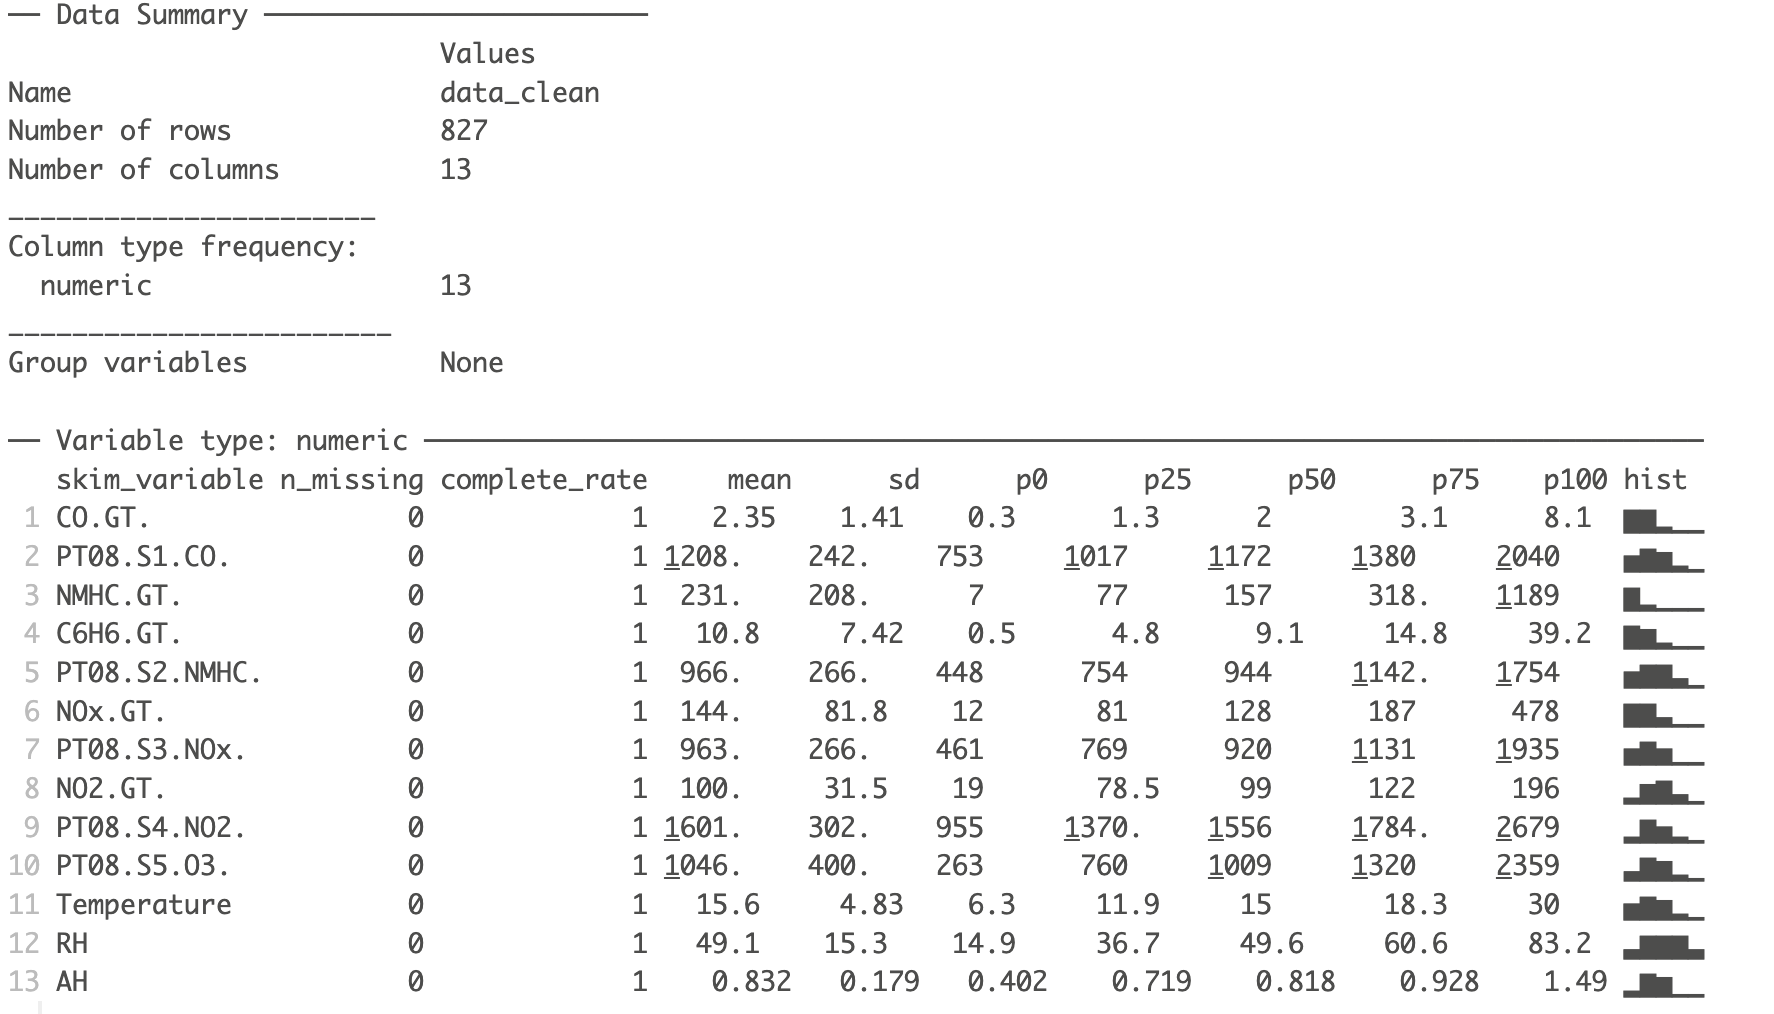
\includegraphics[width=\linewidth]{images/summary_tab2.png}
   \caption{Statistical table (skim)}
   \label{fig:fig1}
\end{figure}

Something intersting in the target variable, the carbon monoxide levels (CO.GT), is that have a wide range, from as low as 0.3 to a high of 8.1, with a mean of 2.35, suggesting significant variability. This may reveal relationships between pollutant concentrations and environmental factors like temperature and humidity.
\newpage
\section{Problem 2}
\subsection{Bad Data Visualization}
We will now look at examples of bad plots and why they are considered such.
In Figure \ref{fig:fig2} and Figure \ref{fig:fig3} we can observe barplots that are heavily influenced by the presence of NA's. In this case, the NA's in the dataset are labelled with the value -200. If they are not purposely removed, they alter the graph and do not allow a clear visualisation of the data.
In Figure \ref{fig:fig4} and Figure \ref{fig:fig5}, on the other hand, we can observe two pie plots representing two numerical variables. This way of representing the data is not optimal for numerical data as the visualisation is not at all clear.
Figure \ref{fig:fig8} represents the boxplot of the variable PT08.S3(NOx). This type of graph can be very useful for identifying outliers and observing the distribution of data. In this situation, the reference scale is not shown, making the data uninterpretable. In addition, the outliers were removed but this was not indicated in any way.
Figure \ref{fig:fig6} and Figure \ref{fig:fig7} are scatter plots where the dots are too large and there are null values that do not allow the data to be displayed correctly.
in Figure \ref{fig:fig9}, the axes are manually scaled, making the representation misleading. Most of the information is not displayed and, if decontextualised, could be used to distort the reality of the data.
Finally, Figure \ref{fig:fig10} presents a histogram that uses few bins, not allowing the distribution of data to be correctly visualised.
\begin{figure}[H]
   \centering
   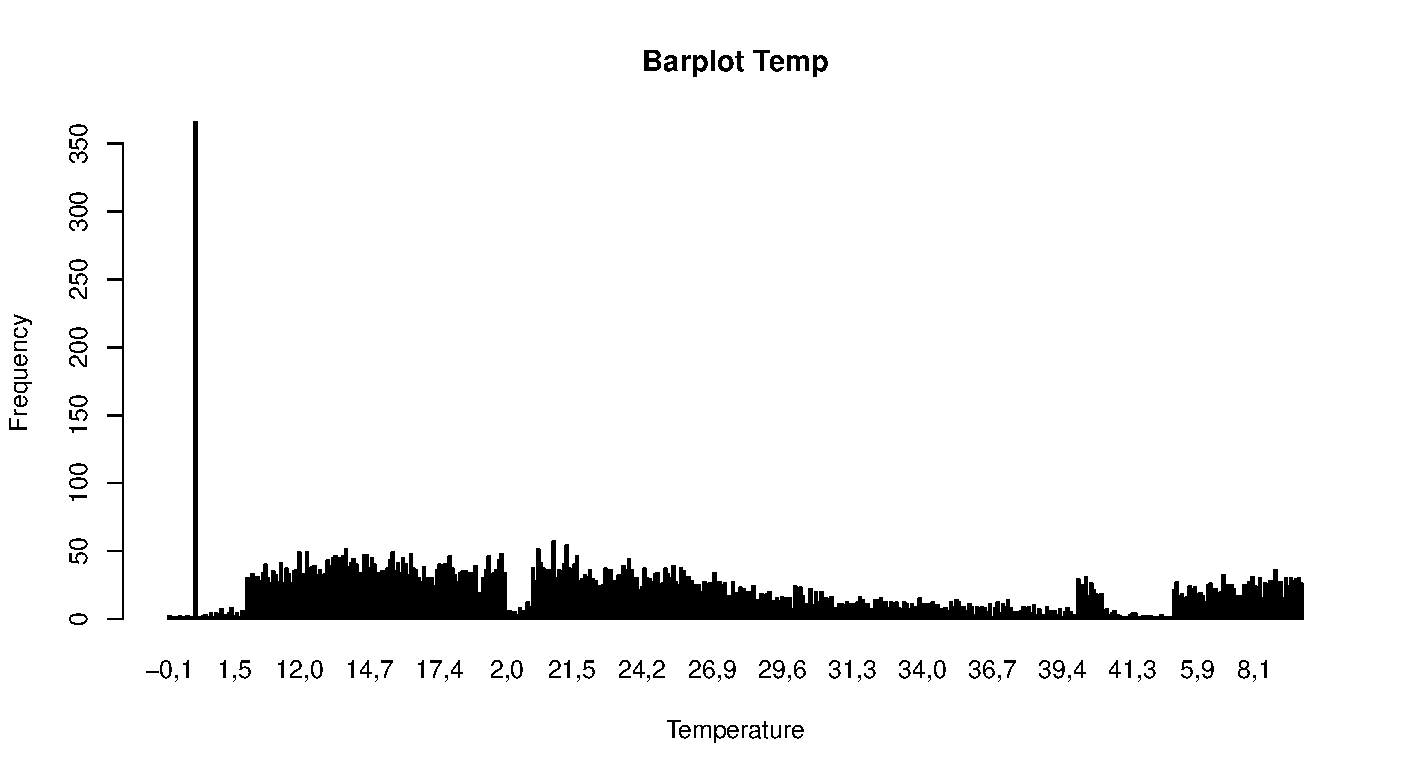
\includegraphics[width=\linewidth]{images/barplottemp.pdf}
   \caption{Barplot of Temperature (chr) variable, with NA's}
   \label{fig:fig2}
\end{figure}
\begin{figure}[H]
   \centering
   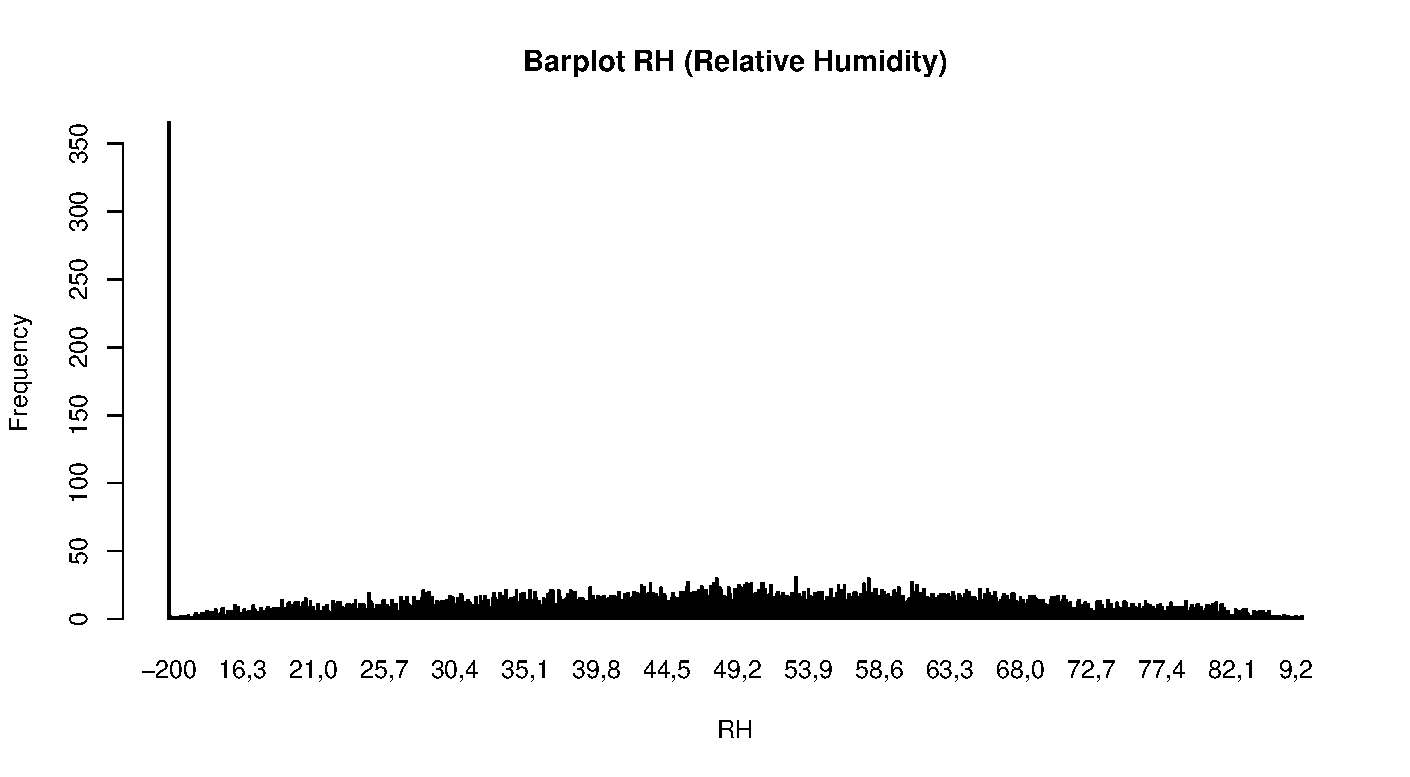
\includegraphics[width=\linewidth]{images/barplotRH.pdf}
   \caption{Barplot of Relative Humidity (chr) variable, with NA's}
   \label{fig:fig3}
\end{figure}
\begin{figure}[H]
   \centering
   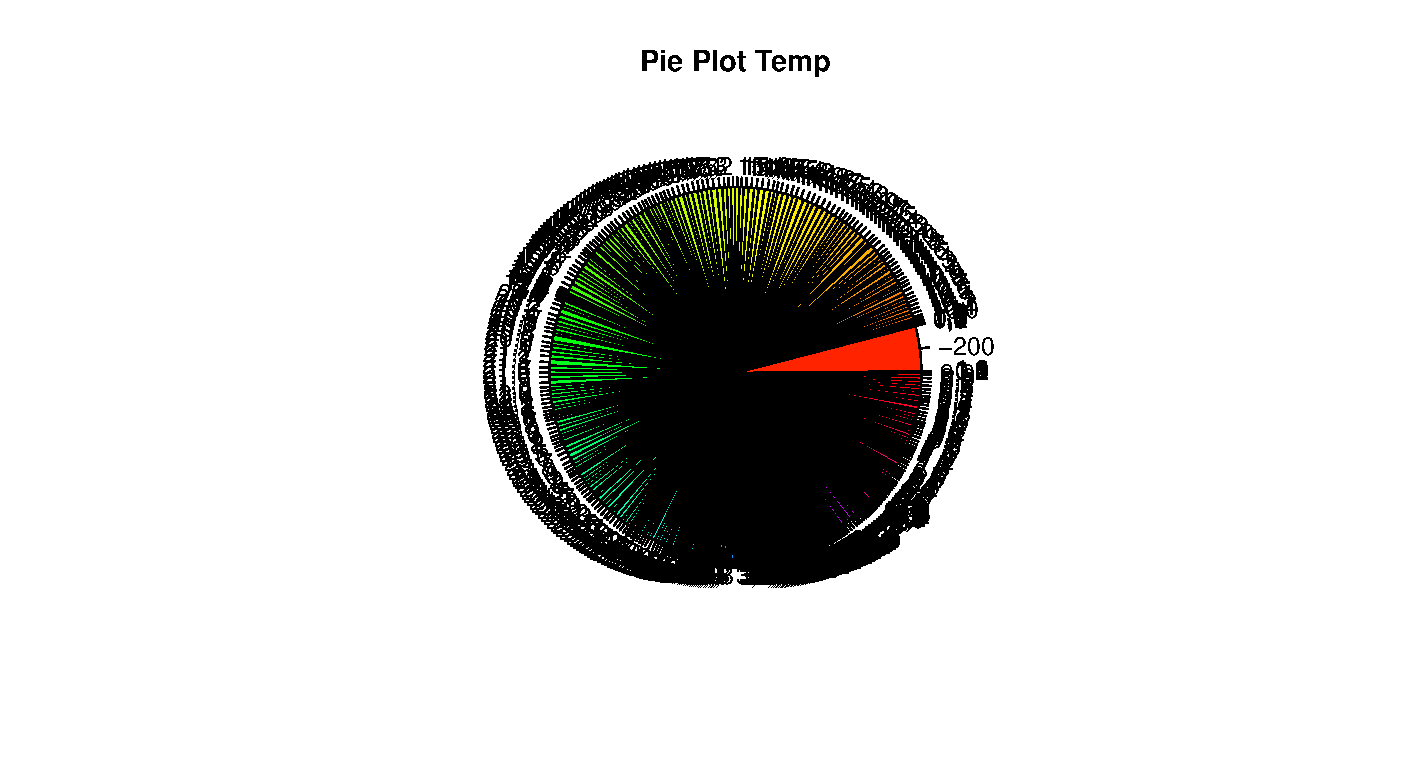
\includegraphics[width=\linewidth]{images/pieplottemp.pdf}
   \caption{Pie Plot of Temperature variable, with NA's}
   \label{fig:fig4}
\end{figure}
\begin{figure}[H]
   \centering
   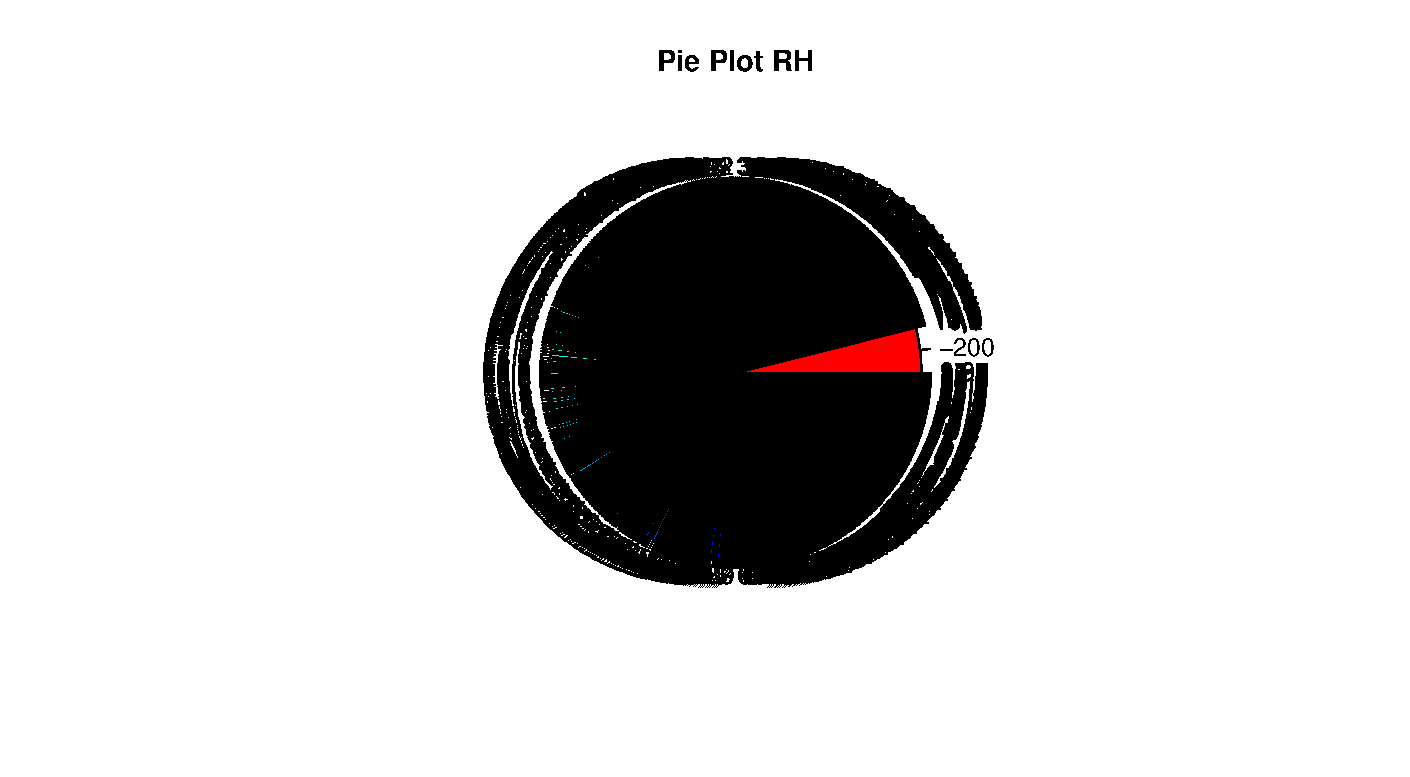
\includegraphics[width=\linewidth]{images/pieplotRH.pdf}
   \caption{Pie Plot of Relative Humidity variable, with NA's}
   \label{fig:fig5}
\end{figure}
\begin{figure}[H]
   \centering
   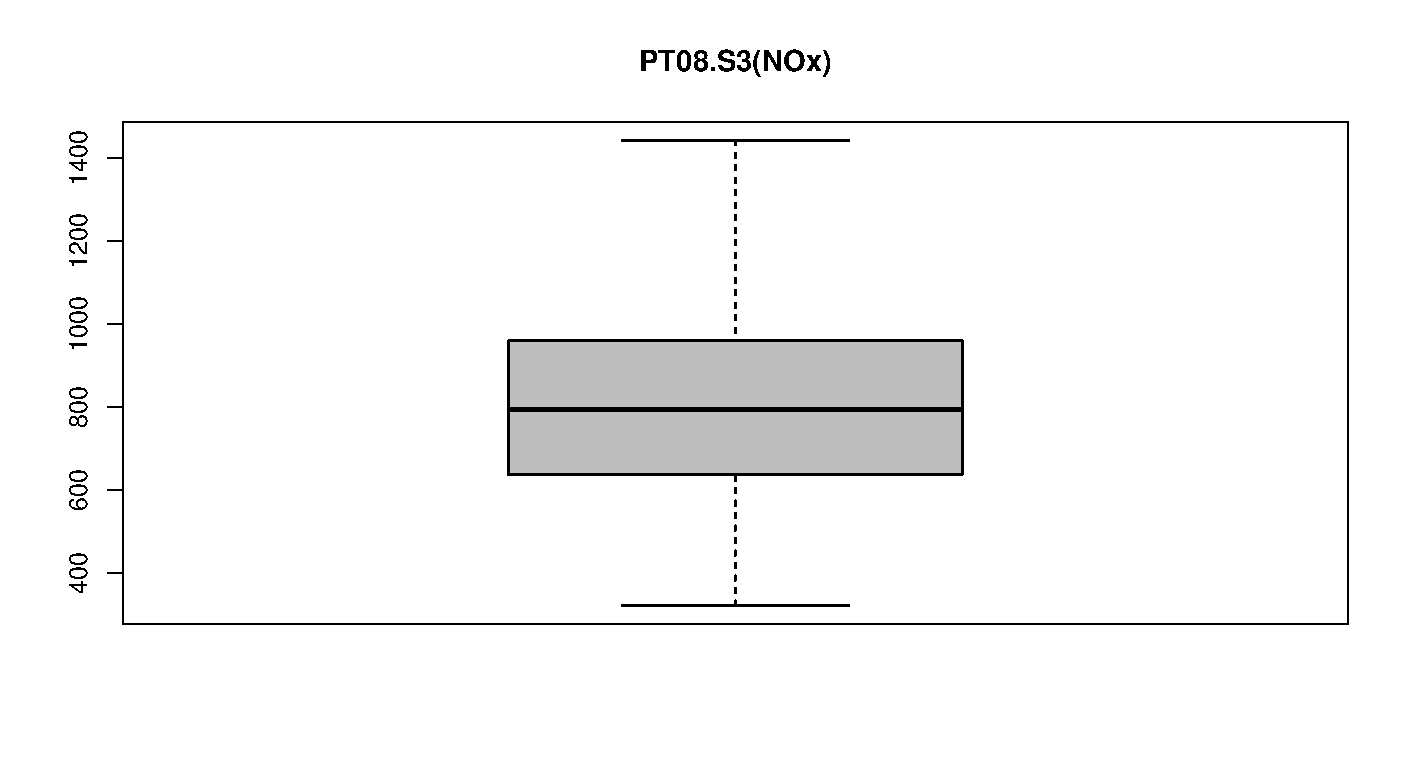
\includegraphics[width=\linewidth]{images/PT08.S3Boxplot.pdf}
   \caption{Boxplot PT08.S3(NOx), but we remove outliers only in the plot}
   \label{fig:fig8}
\end{figure}
\begin{figure}[H]
   \centering
   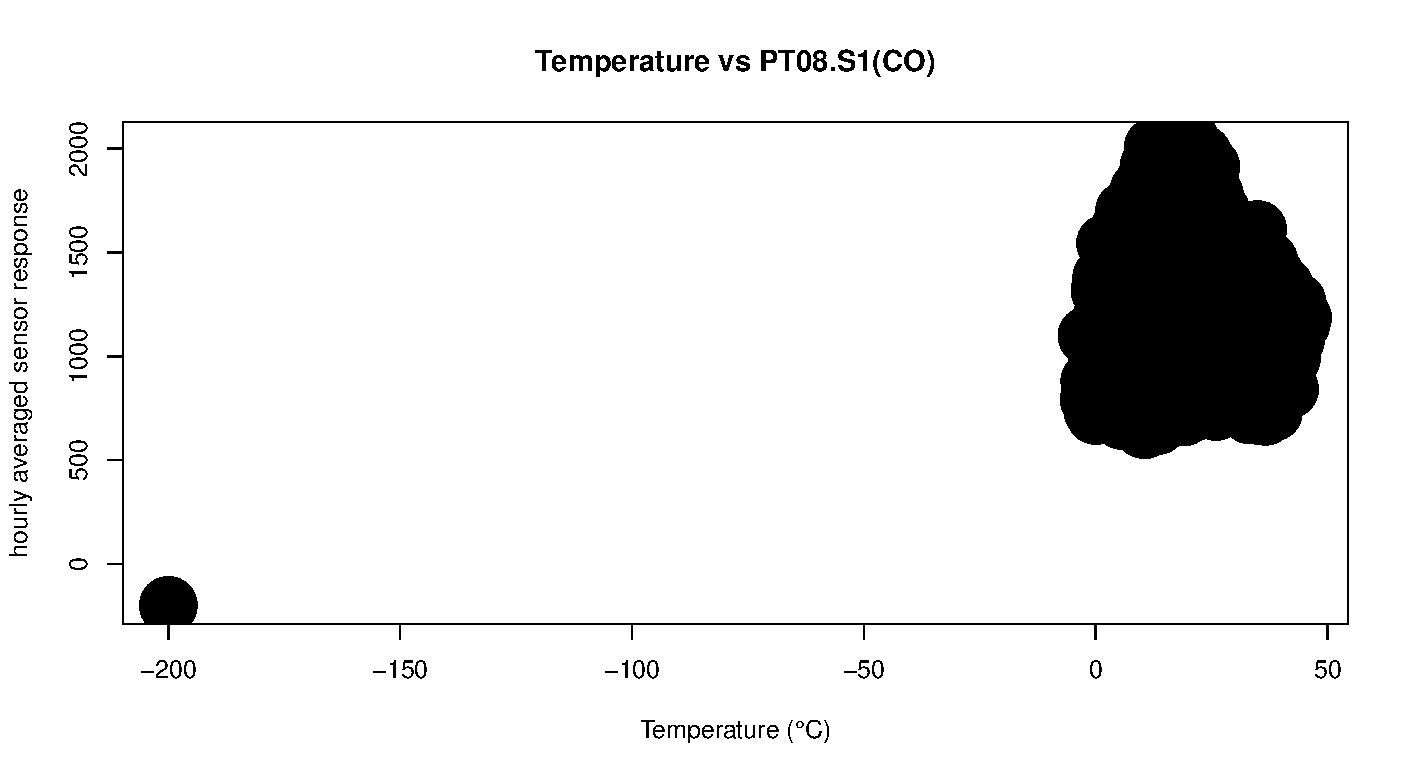
\includegraphics[width=\linewidth]{images/TempvsPT08.pdf}
   \caption{Dumb scatterplot Temperature vs PT08.S1(CO), with NA's}
   \label{fig:fig6}
\end{figure}
\begin{figure}[H]
   \centering
   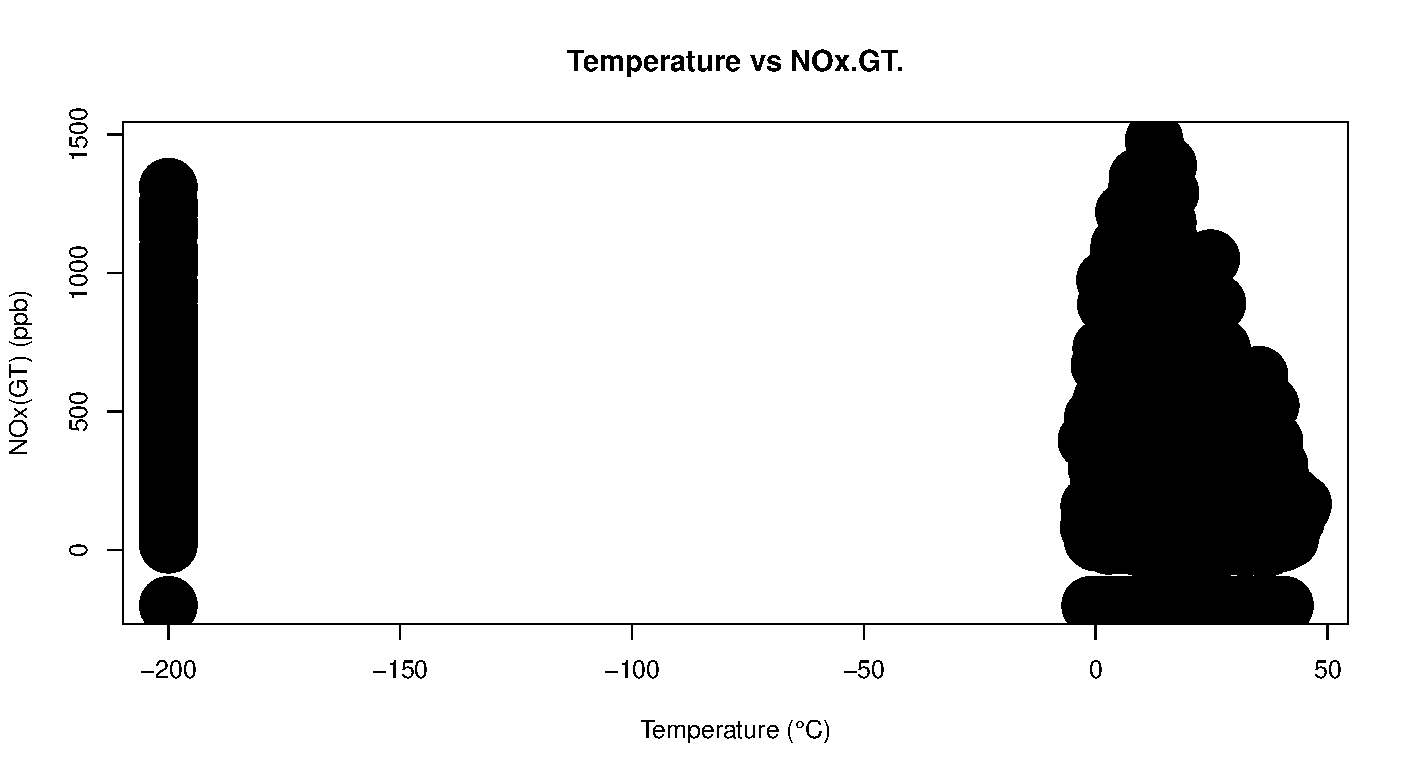
\includegraphics[width=\linewidth]{images/TempvsNOcGT.pdf}
   \caption{Dumb scatterplot Temperature vs NOx.GT., with NA's}
   \label{fig:fig7}
\end{figure}
\begin{figure}[H]
   \centering
   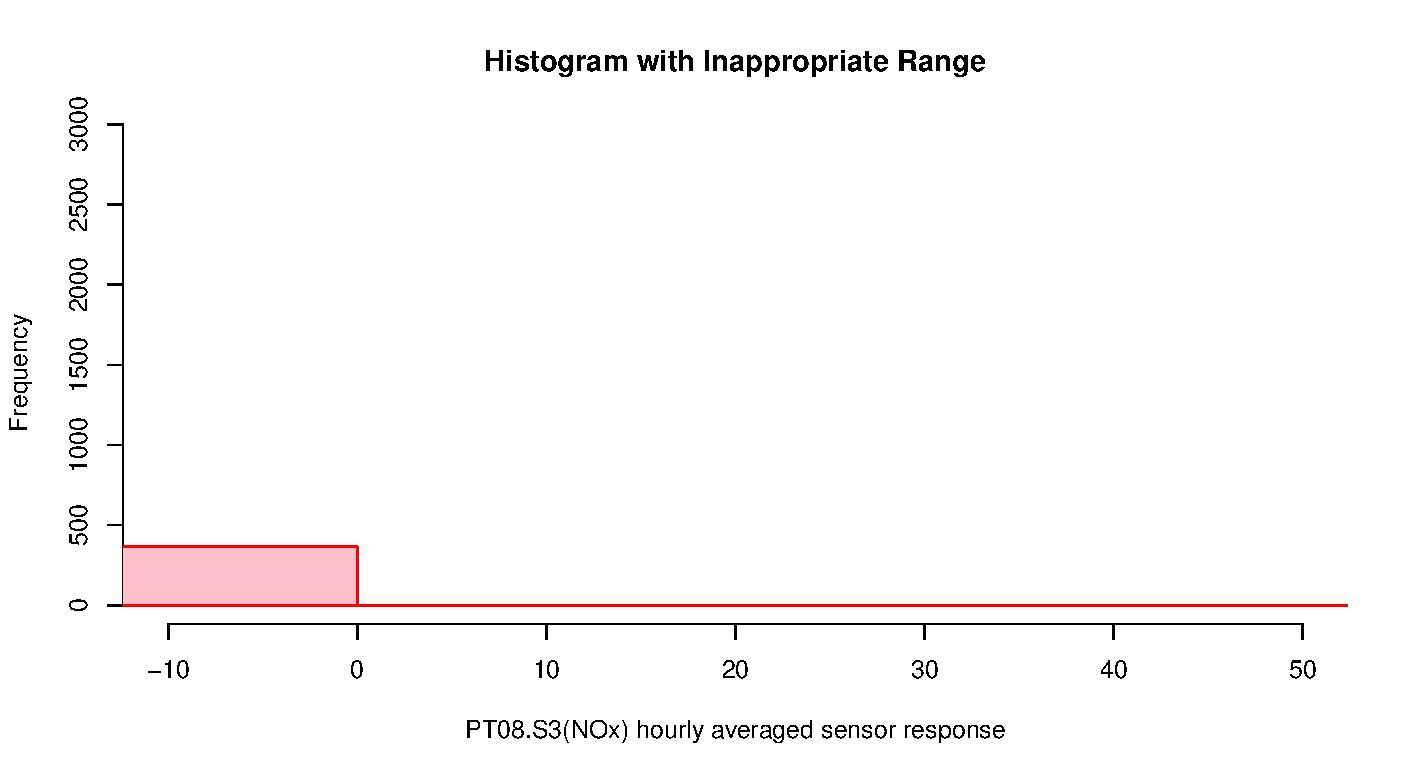
\includegraphics[width=\linewidth]{images/HistInappropRange.pdf}
   \caption{Histogram with (xlim) arbitrary range that may not fit the data}
   \label{fig:fig9}
\end{figure}
\begin{figure}[H]
   \centering
   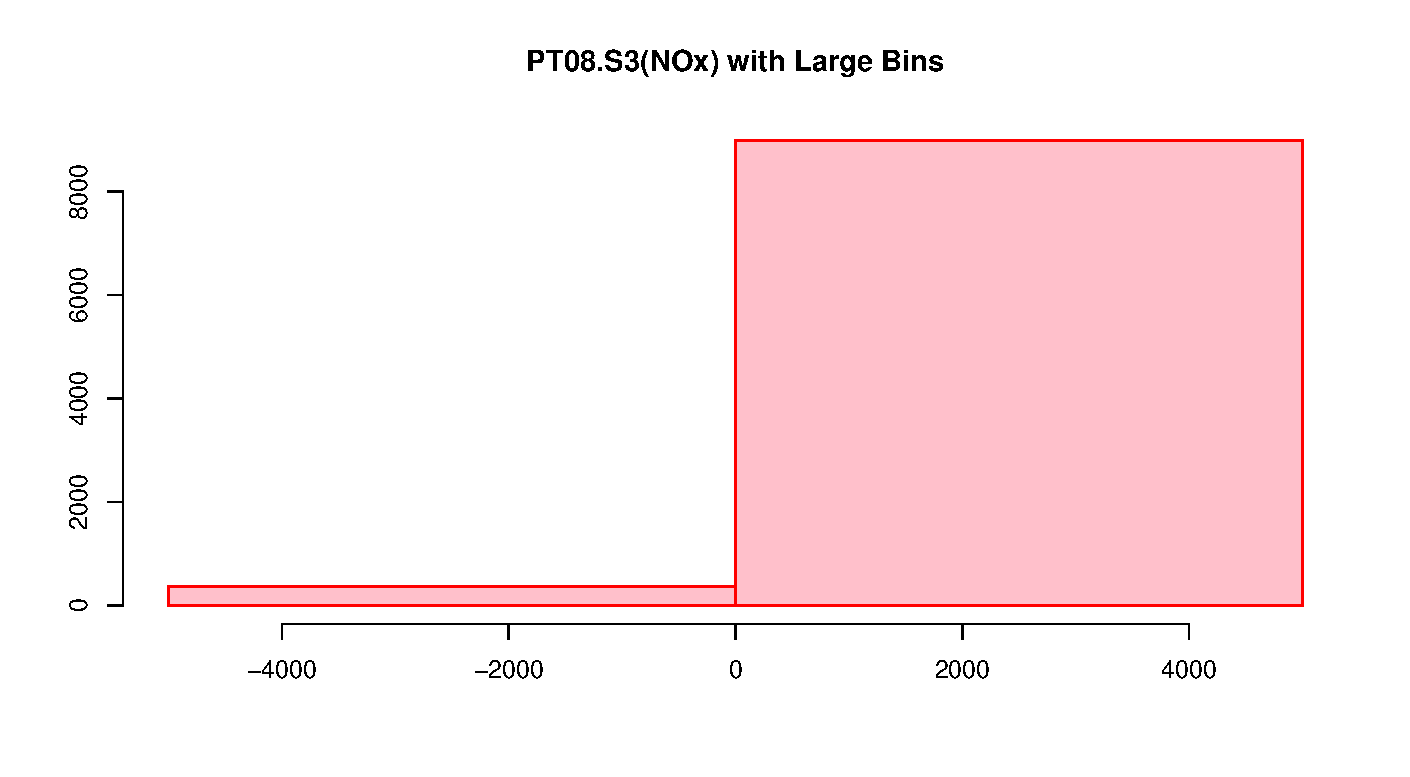
\includegraphics[width=\linewidth]{images/PT08.s3LArgeBins.pdf}
   \caption{Histogram with large bins}
   \label{fig:fig10}
\end{figure}
\section{Problem 3}
\subsection{ Good Data Visualization}
The first substantial change to the graphs was made to the pie charts (e.g. Figure \ref{fig:fig11}), where the categorical variables were grouped in percentage ranges to allow an immediate and effective visualisation of the distribution of character values.
Following the cleaning of the null data, the scatter plots were optimised to be more intuitive for investigating possible relationships between variables, as can be seen in Figure \ref{fig:fig12} and Figure \ref{fig:fig13}. 
By using clean data and optimising the scale of the parameters, the histograms were also optimised, allowing the distribution of individual features to be observed in full (Figure \ref{fig:fig14} and Figure \ref{fig:fig15}).
Finally, the boxplot was also improved, leaving the outliers in the original visualisation and rotating the scale (Figure \ref{fig:fig16}).
\begin{figure}[H]
   \centering
   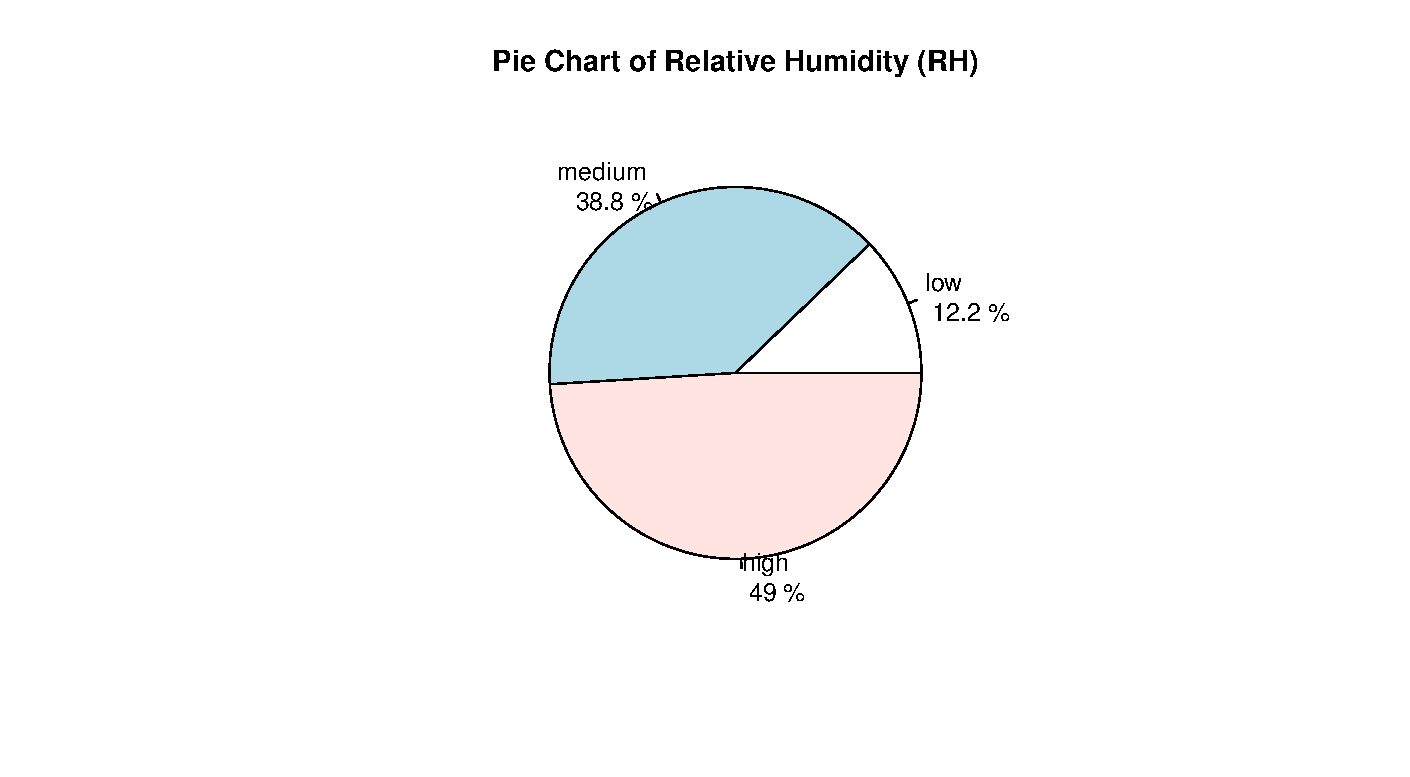
\includegraphics[width=\linewidth]{images/piechartRHgood.pdf}
   \caption{Pie Plot with Range in chr variables}
   \label{fig:fig11}
\end{figure}
\begin{figure}[H]
   \centering
   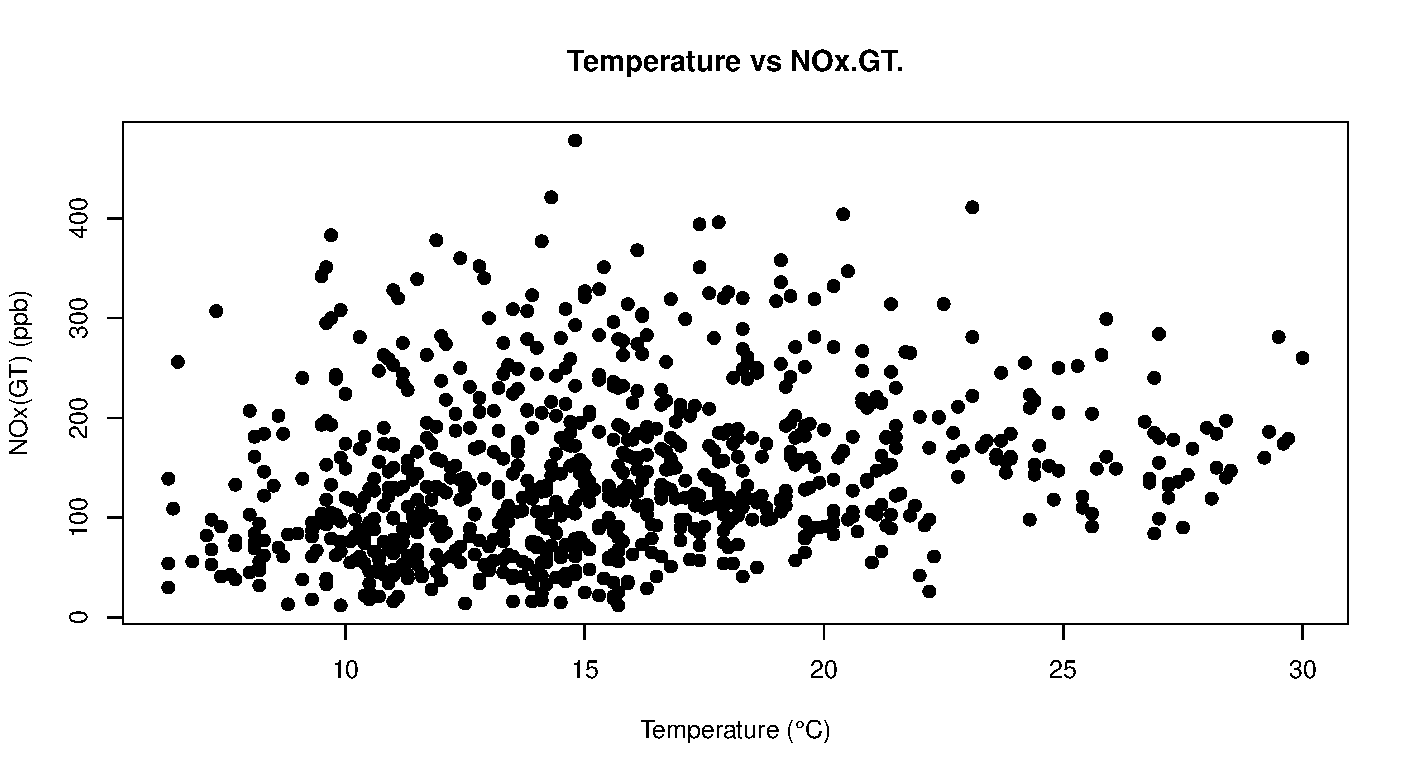
\includegraphics[width=\linewidth]{images/1_r.pdf}
   \caption{Scatterplot Temperature vs NOx(GT)}
   \label{fig:fig12}
\end{figure}
\begin{figure}[H]
   \centering
   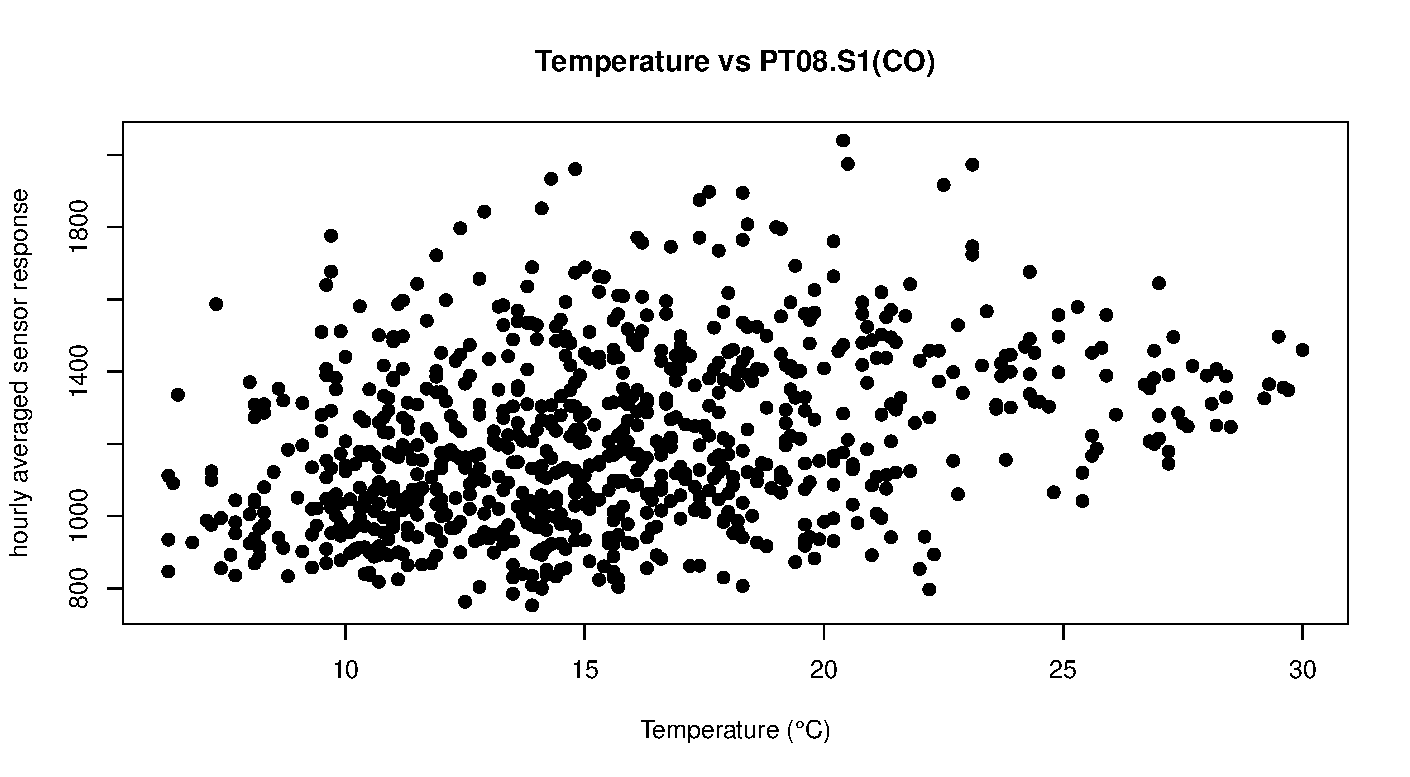
\includegraphics[width=\linewidth]{images/2_r.pdf}
   \caption{Scatterplot Temperature vs PT08.S1(CO)}
   \label{fig:fig13}
\end{figure}
\begin{figure}[H]
   \centering
   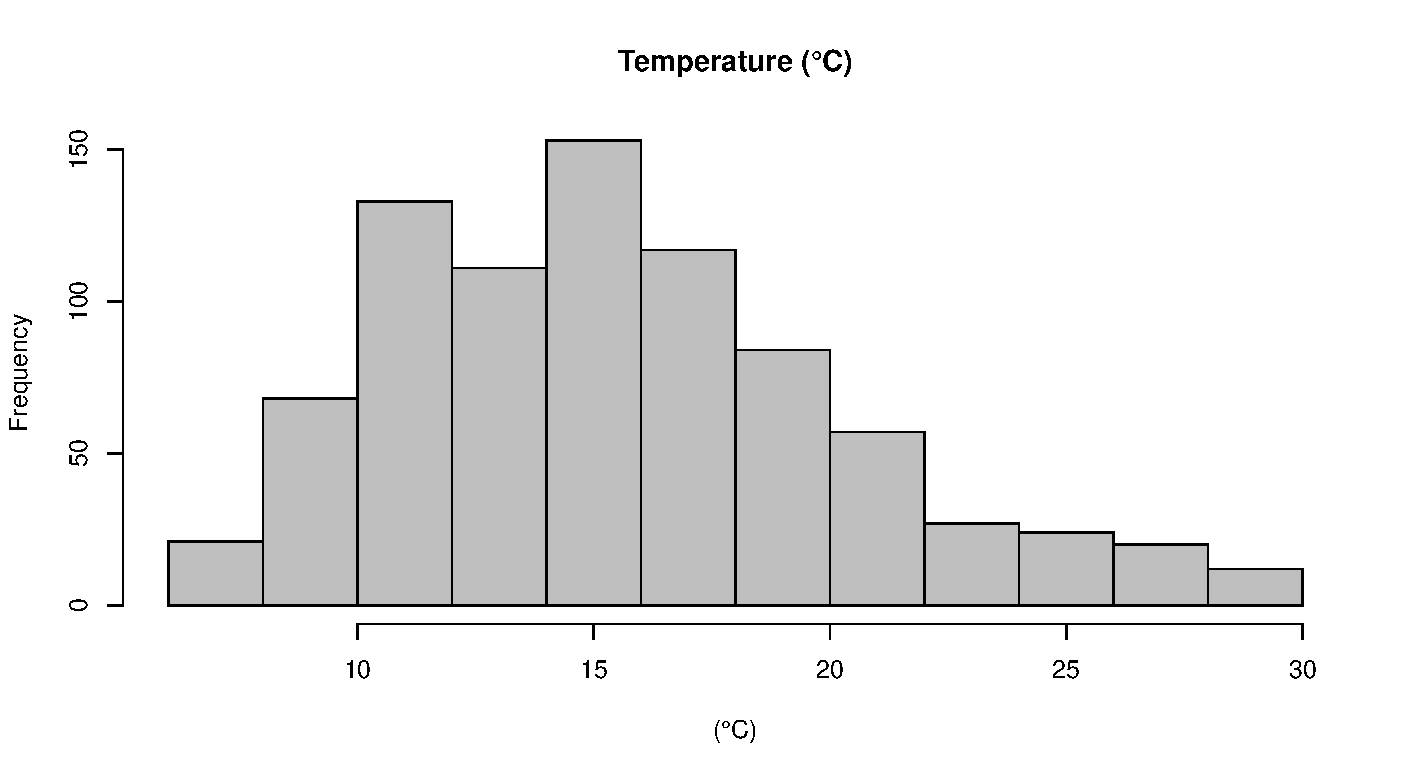
\includegraphics[width=\linewidth]{images/3_r.pdf}
   \caption{Temperature distrib. Histogram}
   \label{fig:fig14}
\end{figure}
\begin{figure}[H]
   \centering
   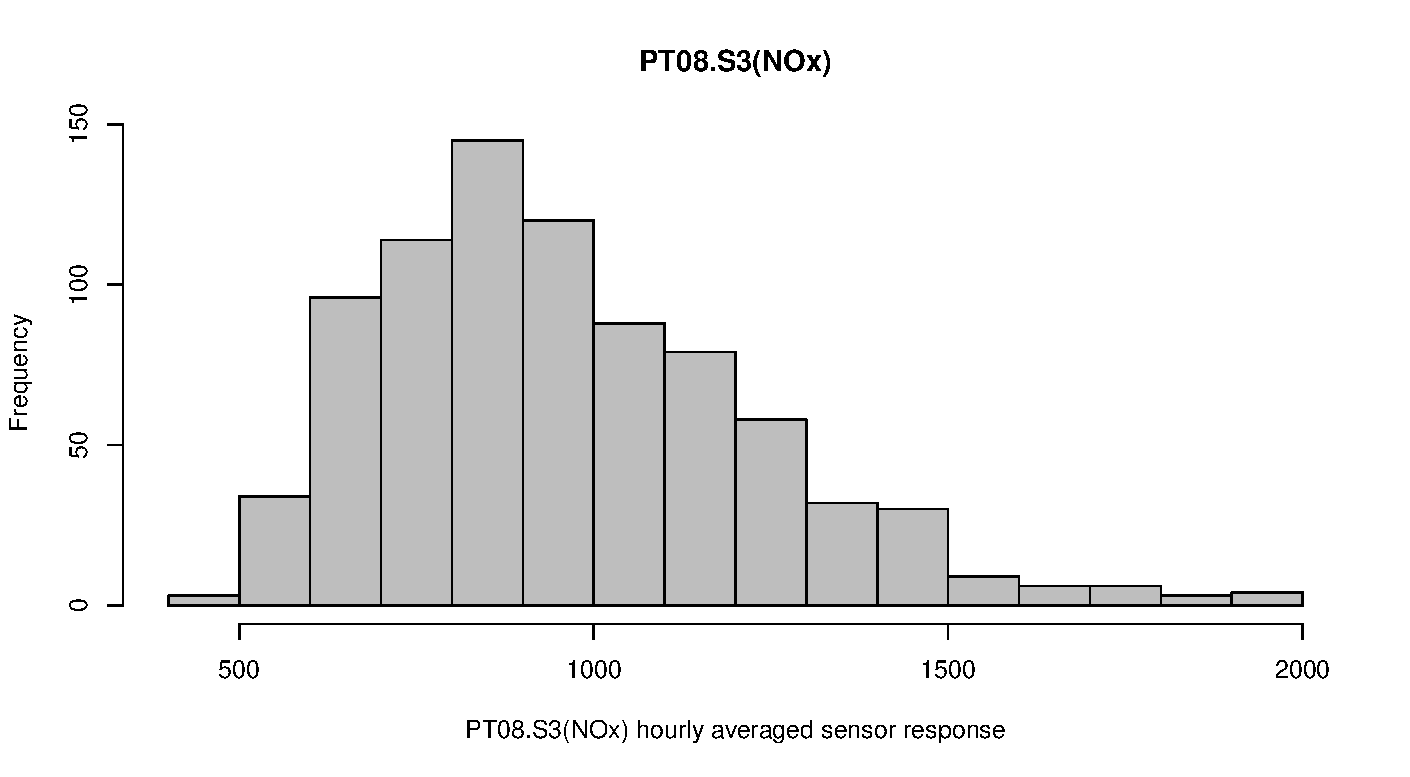
\includegraphics[width=\linewidth]{images/4_r.pdf}
   \caption{PT08.S3(NOx) distrib. Histogram}
   \label{fig:fig15}
\end{figure}
\begin{figure}[H]
   \centering
   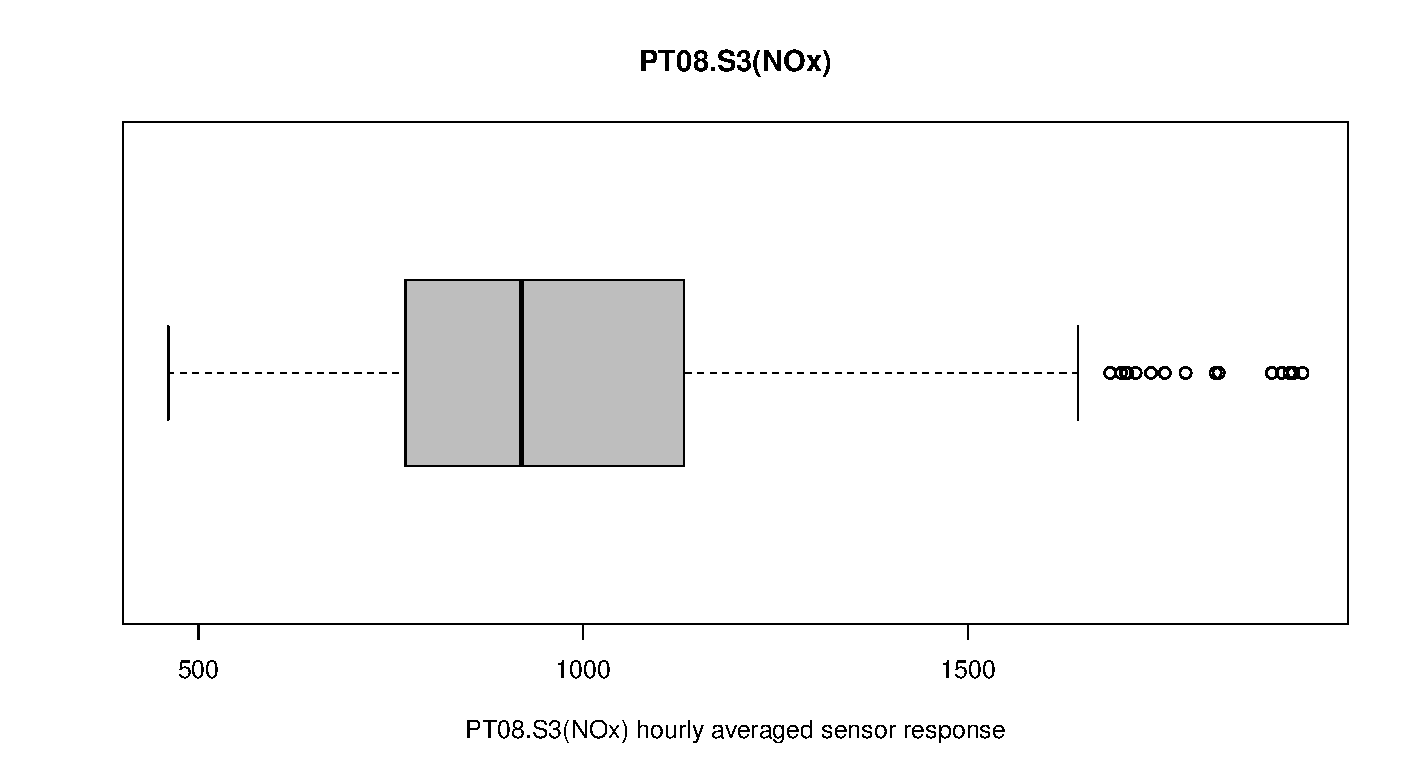
\includegraphics[width=\linewidth]{images/5_r.pdf}
   \caption{PT08.S3(NOx) boxplot}
   \label{fig:fig16}
\end{figure}
\newpage
\section{Problem 4}
\subsection{Simple analysis}
The linear regression model was fitted and the performance was evaluated, yielding a RMSE of 0.25294, indicating a moderate level of predictive accuracy on the dataset.

\begin{figure}[h!]
   \centering
   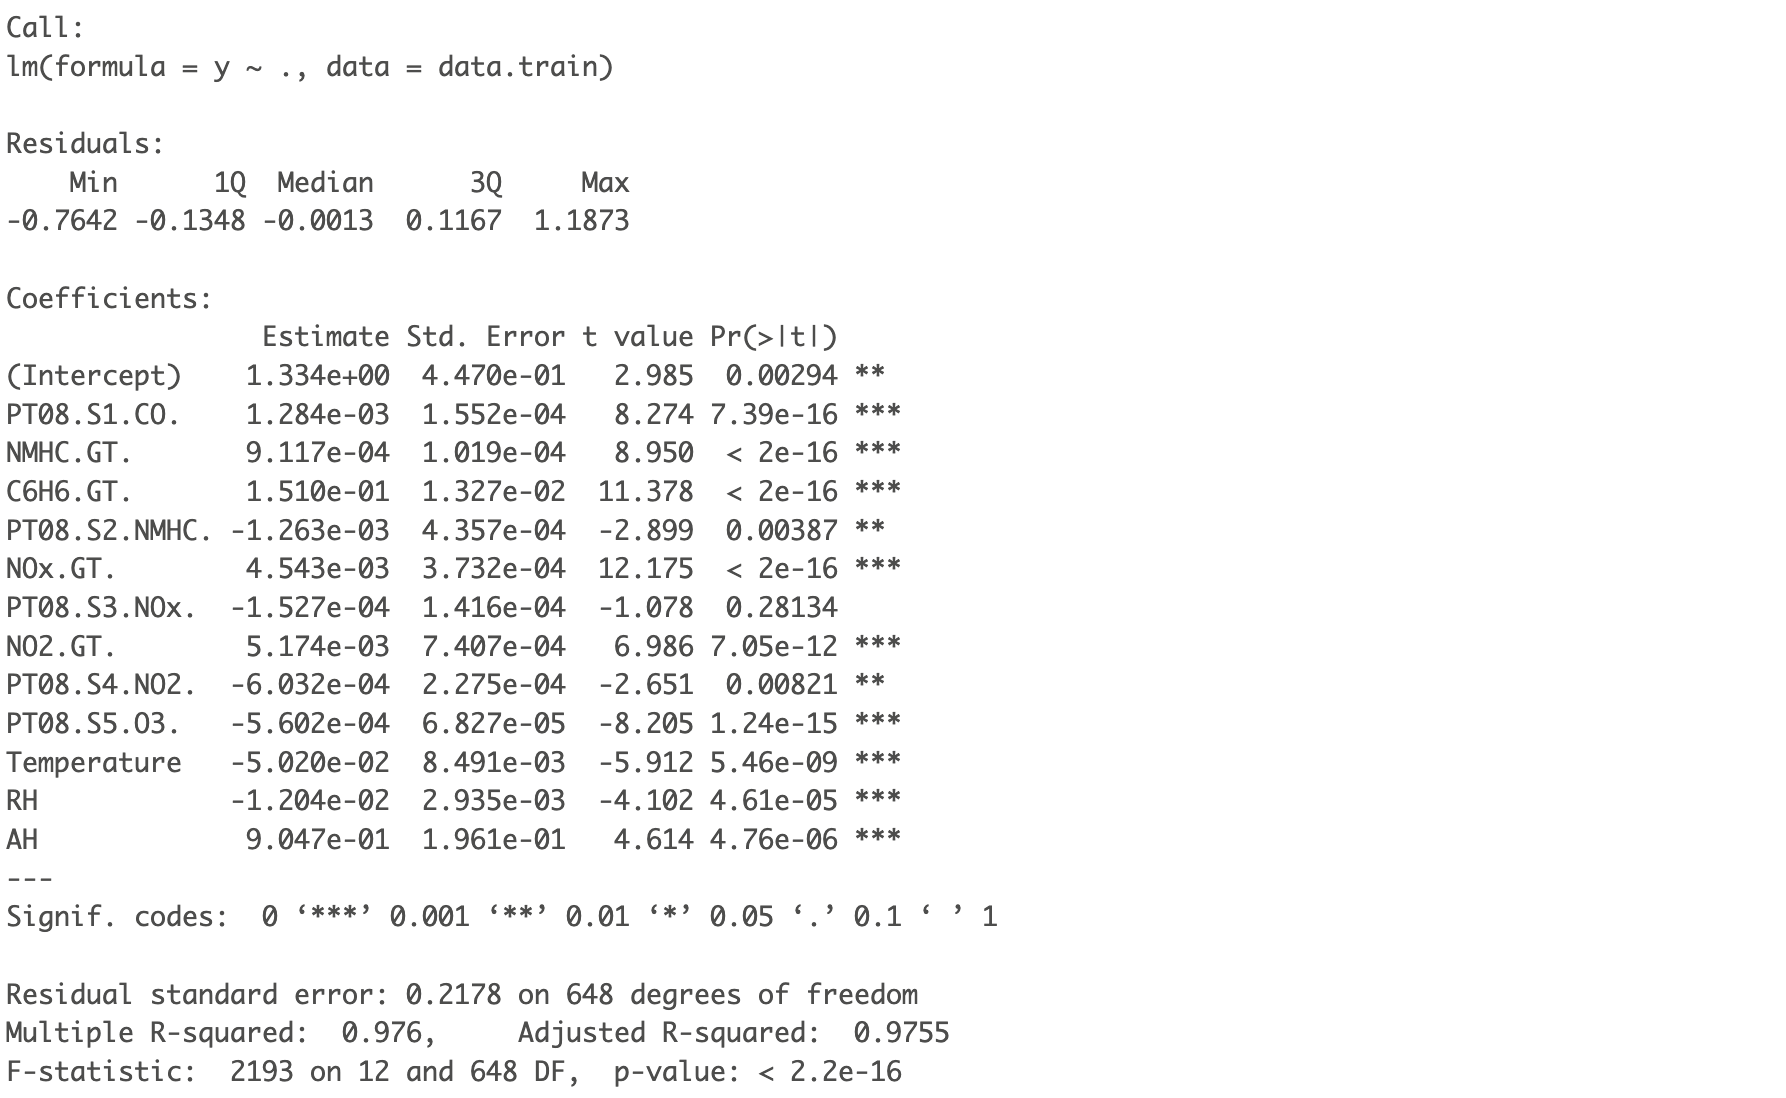
\includegraphics[width=\linewidth]{images/Screenshot 2024-09-17 alle 18.47.02.png}
   \caption{Model summary of the Regression}
   \label{fig:fig17}
\end{figure}
As we can se from Figure \ref{fig:fig17} Most predictors are statistically significant at the 0.05 level, with p-values less than 0.05. These include PT08.S1.CO., NMHC.GT., C6H6.GT., PT08.S2.NMHC., NOx.GT., NO2.GT., PT08.S4.NO2., PT08.S5.O3., Temperature, RH (Relative Humidity), and AH (Absolute Humidity). Notably, many of these variables have extremely small p-values (e.g., < 2e-16), indicating a strong relationship with the target variable. The variable PT08.S3.NOx. has a relatively high p-value (0.28134), indicating that it is not a significant predictor in the model.
The model's R-squared value is 0.976. The adjusted R-squared, which accounts for the number of predictors, is 0.9755, indicating that the model is not overfitting despite the number of predictors.
The residual standard error is 0.2178, this error seems relatively low, suggesting that the model has a good fit to the training data. The RMSE value of 0.25294 further indicates the model's predictive accuracy.
\begin{figure}[H]
   \centering
   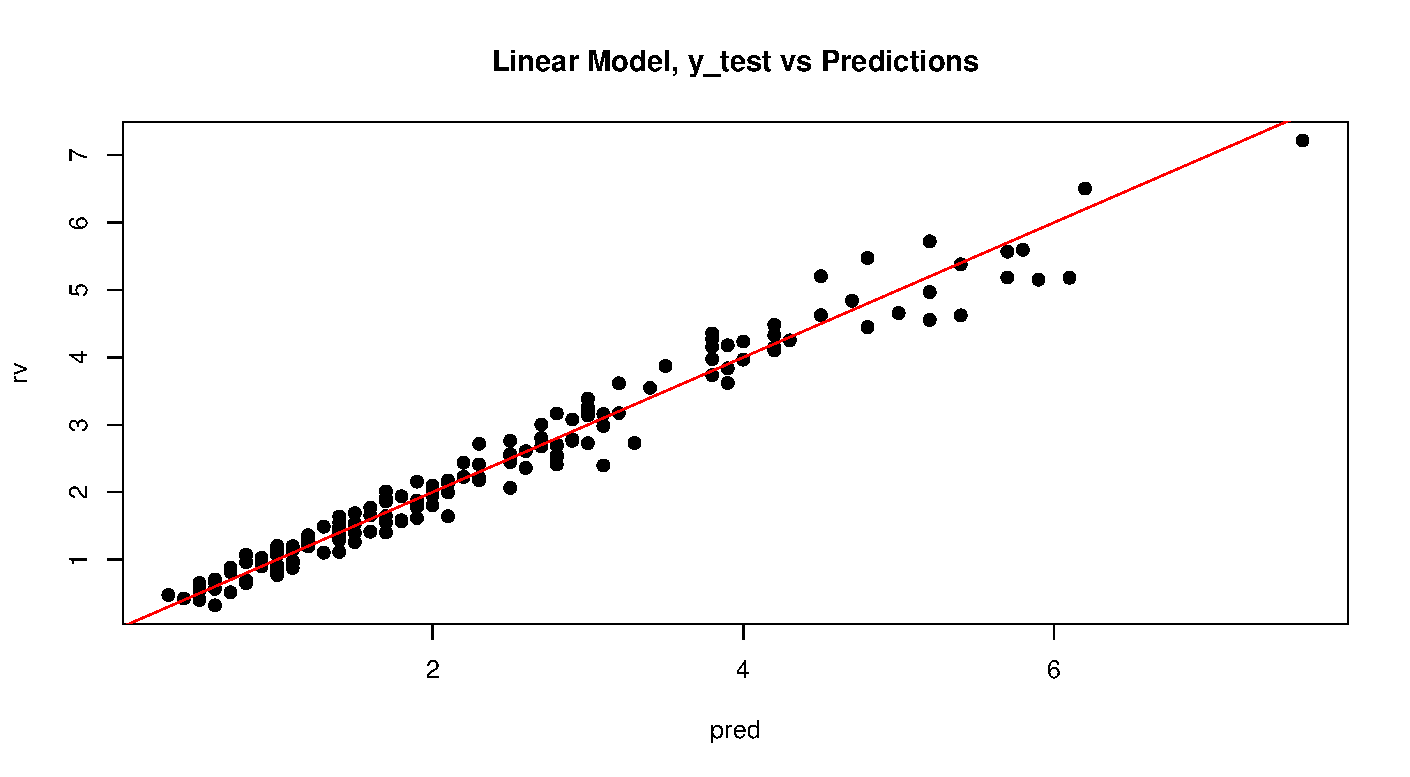
\includegraphics[width=\linewidth]{images/linear_model.pdf}
   \caption{Regression predictions}
   \label{fig:fig18}
\end{figure}
Figure \ref{fig:fig18} shows the graphical representation of the predicted values and the test values. 
In addition to simple linear regression, we now perform model selection to look at the covariates.
\begin{figure}[H]
   \centering
   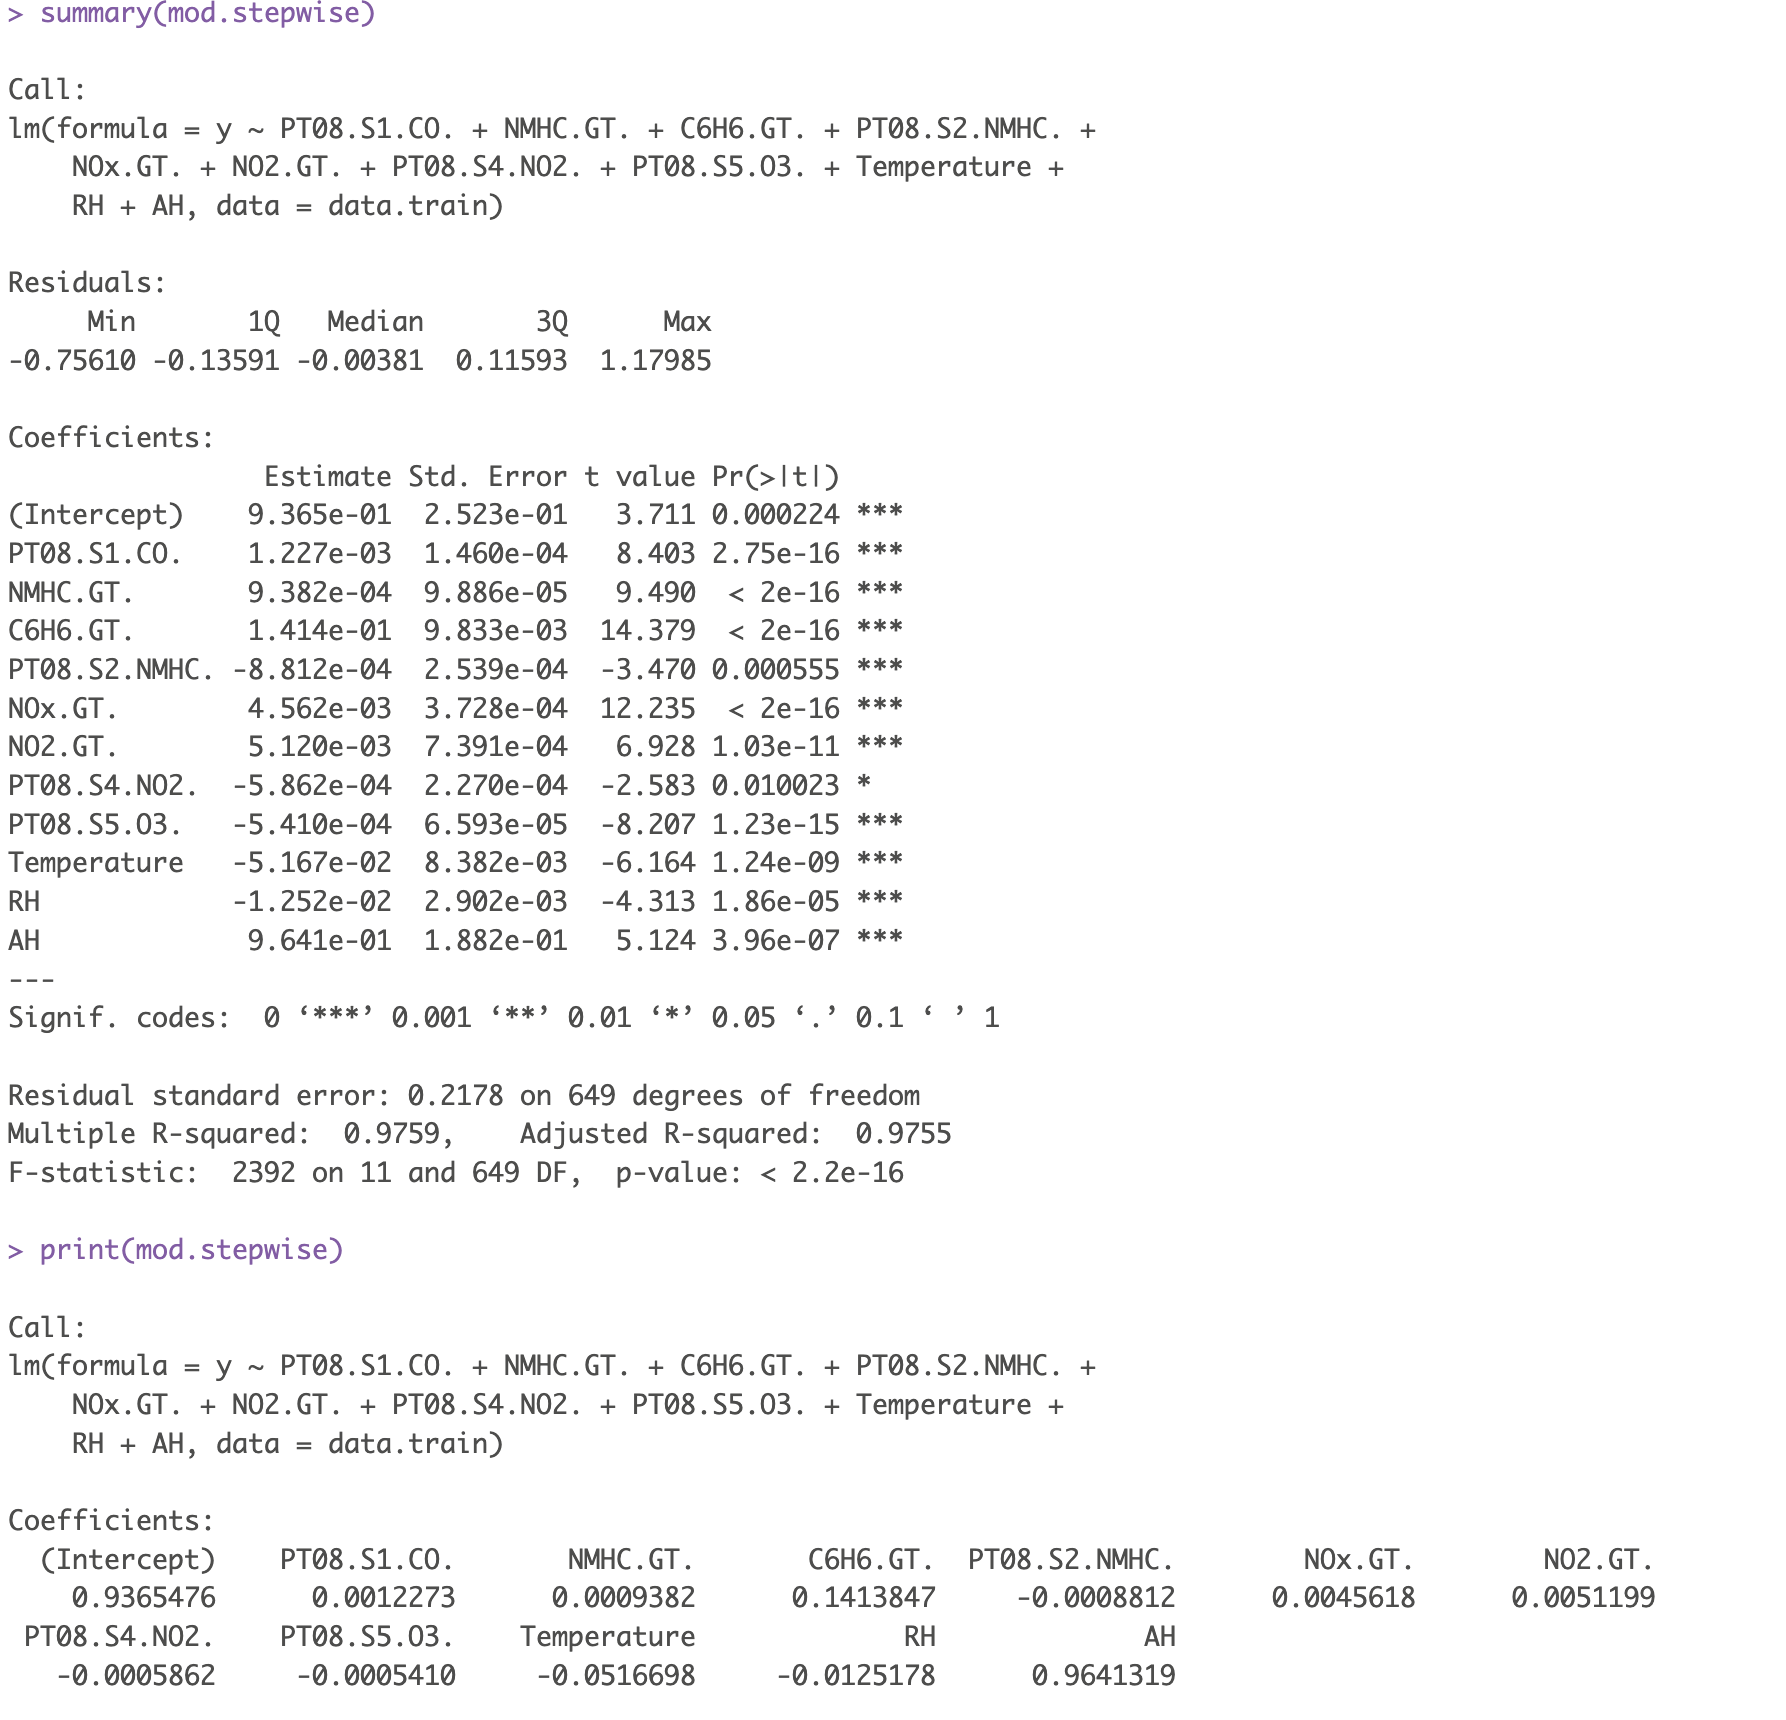
\includegraphics[width=\linewidth]{images/stepwise.png}
   \caption{Model selection: Stepwise}
   \label{fig:fig19}
\end{figure}
Using the stepwise method (Figure \ref{fig:fig19}) to find a model that balances the complexity and explanatory power of the data, we obtain a model similar to that of simple regression with the removal of a variable (PT08.S3(NOx)) that had already been identified as not statistically significant.
\begin{figure}[H]
   \centering
   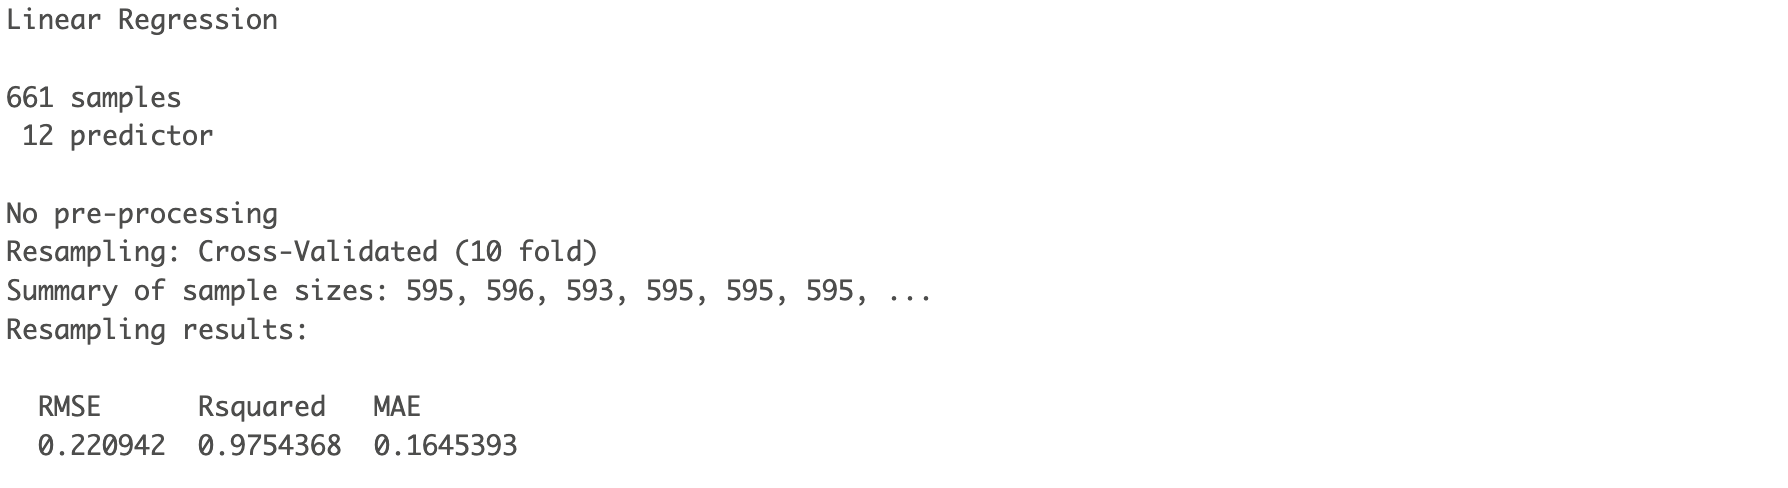
\includegraphics[width=\linewidth]{images/cv.png}
   \caption{Model selection: Cross Validation}
   \label{fig:fig20}
\end{figure}
Through the cross-validation performed in Figure \ref{fig:fig20} the model appears to have a very good predictive ability on the basis of cross-validation, but it is important to bear in mind the risk of overfitting and to evaluate the model further on a separate test dataset.
\subsection{Conclusions}
The linear regression model appears to be adequate for this dataset.
This conclusion is supported by the high values of $\mathbf{R^2}$ and adjusted $\mathbf{R^2}$, indicating that the model explains a significant portion of the variance in the response variable.
Additionally, the statistical significance of the predictors and the low residual standard error suggest that the model is both appropriate and sufficiently accurate in capturing the relationships within the data. 
However, the high $\mathbf{R^2}$ value raises a potential concern for overfitting. Nevertheless, cross-validation results demonstrate good performance on unseen data, suggesting that the risk of overfitting is appropriately managed. We can say that the linear regression model seems suitable for this dataset, owing to its strong explanatory power and the statistical significance of the included variables.
If we look at the $\mathbf{RMSE}$ of our linear model, in general it's very small. This means that, on average, the model predictions are close to the actual observed values, indicating good predictive accuracy in an absolute sense.
\newpage
\section{Additional models}
After training a linear regression model, it is advisable to evaluate Lasso and Ridge regression as well, primarily due to their regularization properties. Linear regression can suffer from issues like overfitting and multicollinearity. Lasso and Ridge address these issues by introducing a penalty to the regression objective. Both methods help in controlling the bias-variance trade-off by tuning a regularization parameter, leading to models with enhanced generalization capability. Those models can yield more robust and parsimonious models, especially in high-dimensional settings.
\subsection{Ridge}
The Ridge regression was performed using the glmnet function. The lambda value here is relatively low that implies that the regularization penalty (which shrinks the coefficients towards zero) is mild.
This basically means that the model does not need much regularization to fit the data well. the predictors might not be suffering significantly from issues like multicollinearity or overfitting.
\begin{figure}[H]
   \centering
   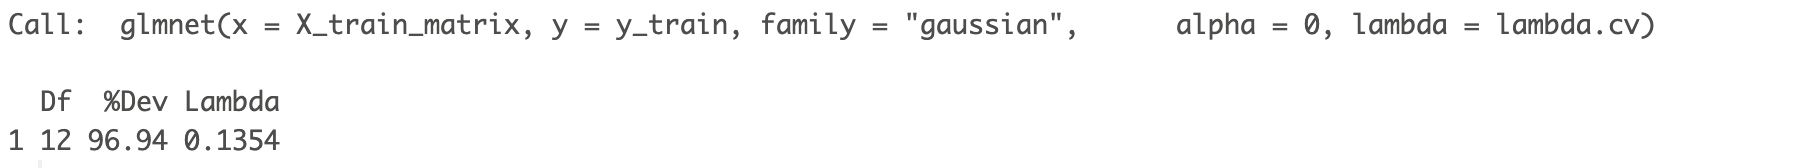
\includegraphics[width=\linewidth]{images/ridge.png}
   \label{fig:fig21}
\end{figure}
\subsection{Lasso}
The lambda value in the Lasso model is even lower. This tiny value suggests that the model requires minimal regularization to achieve optimal performance.
The predictors included by Lasso might already have a strong relationship with the response variable, and the regularization serves only to fine-tune their influence slightly
\begin{figure}[H]
   \centering
   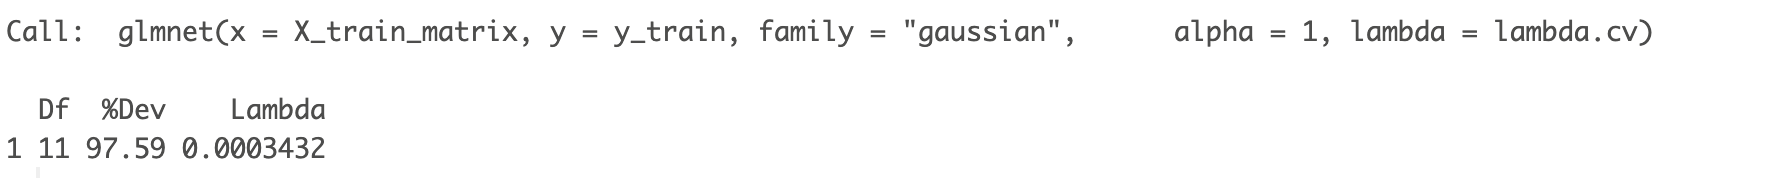
\includegraphics[width=\linewidth]{images/lasso.png}
   \label{fig:fig22}
\end{figure}
\subsection{Lambda approaches zero}
\subsubsection{1. Ridge Regression}
Objective function Ridge regression:
\[
\min_{\boldsymbol{\beta}} \left\{ \sum_{i=1}^{n} (y_i - \mathbf{x}_i^T \boldsymbol{\beta})^2 + \lambda \sum_{j=1}^{p} \beta_j^2 \right\},
\]
When \(\lambda \to 0\):
\[
\lim_{\lambda \to 0} \left\{ \sum_{i=1}^{n} (y_i - \mathbf{x}_i^T \boldsymbol{\beta})^2 + \lambda \sum_{j=1}^{p} \beta_j^2 \right\} = \sum_{i=1}^{n} (y_i - \mathbf{x}_i^T \boldsymbol{\beta})^2.
\]
This is the objective function of the OLS regression, which minimizes the sum of squared residuals:
\[
\min_{\boldsymbol{\beta}} \sum_{i=1}^{n} (y_i - \mathbf{x}_i^T \boldsymbol{\beta})^2.
\]

Therefore, when \(\lambda \to 0\), Ridge regression reduces to the OLS regression.
\subsubsection{Lasso Regression}
Objective function Lasso regression:
\[
\min_{\boldsymbol{\beta}} \left\{ \sum_{i=1}^{n} (y_i - \mathbf{x}_i^T \boldsymbol{\beta})^2 + \lambda \sum_{j=1}^{p} \|\beta_j\| \right\}.
\]
When \(\lambda \to 0\):
\[
\lim_{\lambda \to 0} \left\{ \sum_{i=1}^{n} (y_i - \mathbf{x}_i^T \boldsymbol{\beta})^2 + \lambda \sum_{j=1}^{p} |\beta_j| \right\} = \sum_{i=1}^{n} (y_i - \mathbf{x}_i^T \boldsymbol{\beta})^2.
\]
Again, this is the objective function of the OLS regression:
\[
\min_{\boldsymbol{\beta}} \sum_{i=1}^{n} (y_i - \mathbf{x}_i^T \boldsymbol{\beta})^2.
\]
Therefore, when \(\lambda \to 0\), Lasso regression also reduces to the OLS regression.
\subsection{Conclusions}
The fact that both models have low lambda values implies that the dataset's linear relationships are already relatively well-behaved. For an ordinary linear regression model (without any regularization), this suggests that the predictors might not be overly collinear, and the model does not suffer much from overfitting. Essentially, the underlying linear model fits the data quite well even without regularization.

\end{document}
